\section{Results and Discussion}
% Structure with subsections
% Use of figures/tables (max. 5)
% General description of the results
\subsection{Differentially Expressed Genes and Network Creation}

Under the chosen thresholds discussed in section \ref{sec:methods-deg}, 908 genes were found to be differentially expressed (495 up-regulated and 413 down-regulated). STRING could query 828 of them; using other ID types did not change this. After querying the additional EDS-related genes, the resulting network consists of 847 genes and 6129 connections. The position of the known EDS genes in the network is, on average, more central than expected by chance based on degree, clustering coefficient, betweenness centrality and closeness centrality, supporting the close relationship between hEDS and other EDS types.

\subsection{Gene Ontology and clustering}

GO-enrichment is performed on the DEGs to acquire an overview of over-represented molecular functions, biological processes, and cellular components. In contrast to later results, which include the known EDS genes, this analysis is performed purely on the differentially expressed genes. The over-representation analysis shows terms related to chromatin, nucleosomes, the cell cycle signalling and regulation and the chromosomal region. The exact GO terms are shown in Table \ref{table:go-all-DEG} and are generally consistent with findings of previous research \cite{Chiarelli2018, Ritelli2022, Gensemer2021}.

%Biological processes over-represented in the DEGs include cell-cycle regulation, signalling and transition, nucleosome assembly and organisation and protein-DNA assembly and organisation.  Cellular components affected are the nucleosome (GO:0000786), the chromosomal region (GO:0098687 and GO:0000775), the protein-DNA complex (GO:0032993) and the collagen-containing extracellular matrix (ECM) (GO:0062023). Over-representation analysis for the molecular function is less meaningfull on a large network. Still, three terms are related to a significantly higher number of genes than the rest: The structural constituent of chromatin (GO:0030527), protein heterodimerization activity (GO:0046982) and extracellular matrix structural constituent (GO:0005201).

\begin{table}[hbt]
	\centering
	\begin{subtable}[h]{0.49\textwidth}
		\centering
  		\begin{tabular}{r|p{4cm}}
    		\textbf{GO term} & \textbf{Description}\\
    		\hline
    		GO:0030527 & structural constituent of chromatin\\
    		GO:0046982 & protein heterodimerization activity\\
    		GO:0005201 & extracellular matrix structural constituent\\
  		\end{tabular}
  		\caption{Molecular Function}
  	\end{subtable}
  	\hfill
  	\begin{subtable}[h]{0.49\textwidth}
  		\centering
  		\begin{tabular}{r|p{4cm}}
  		 \textbf{GO term} & \textbf{Description}\\
  		 \hline
  		 GO:0000786 & nucleosome \\
  		 GO:0032993 & protein-DNA complex \\
  		 GO:0098687& chromosomal region\\
  		 GO:0000775 & chromosome, centromeric region\\
  		 GO:0062023 & collagen-containing extracellular matrix\\
  		\end{tabular}	
  		\caption{Cellular Component}
  	\end{subtable}
  	\hfill
  	\begin{subtable}[t]{\textwidth}
  		\centering
  		\begin{tabular}{r|p{8cm}}
  		 \textbf{GO term} & \textbf{Description}\\
  		 \hline
  		 GO:0006334 & nucleosome assembly \\
  		 GO:0034728 & nucleosome organization \\
  		 GO:0065004 & protein-DNA complex assembly\\
  		 GO:0071824 & protein-DNA complex organization \\
  		 GO:0000075 & cell cycle checkpoint signaling\\
  		 GO:1901988 & negative regulation of cell cycle phase transition\\
  		 GO:0010948 & negative regulation of cell cycle process\\
  		 GO:0045786 & negative regulation of cell cycle\\
  		\end{tabular}	
  		\caption{Biological Process}
  	\end{subtable}
  	\hfill
  	\vfill
  \caption{GO terms for the differentially expressed genes.}
  \label{table:go-all-DEG}
\end{table}

%Pathway enrichment is performed against the KEGG database \cite{KEGG}. The results are displayed in Figure \ref{fig:kegg-pathways}. [TODO: Analysis]
%
%\begin{figure}
%	\centering
%	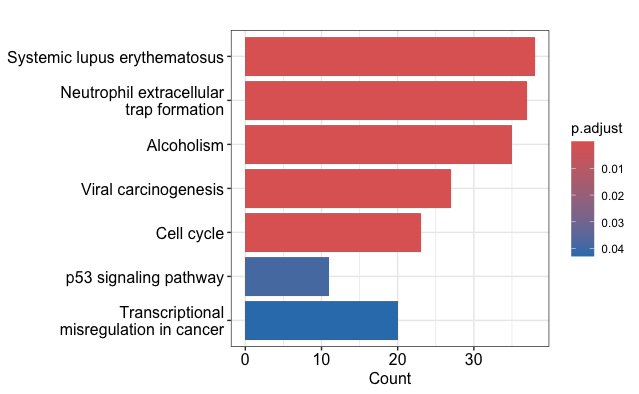
\includegraphics[width=0.8\textwidth]{fig/pathways-kegg.png}
%	\caption{TODO}
%	\label{fig:kegg-pathways}
%\end{figure}



\subsubsection{MCODE}
Running MCODE on the created networks finds 3 clusters with more than 15 genes, one with 66 genes and 1953 connections, one with 44 genes and 686 connections and one with 16 genes and 114 connections, with the two larger clusters containing up-regulated genes only and no genes known to cause other EDS types. % TODO: interpretation - might those be processes that we see only in hEDS and not in other EDS types? Look at heat in community cluster

\paragraph{MCODE cluster with EDS genes.}
The third, smaller cluster, shown in Figure \ref{fig:mcode3}, contains mainly up-regulated genes, including eight EDS-related genes with no significant differential expression and nine differentially expressed genes. One of the EDS genes is also one of the two down-regulated genes. Notably, all EDS genes besides ADAMTS2 exhibit high Closeness Centrality, consistent with EDS genes being more central in the complete network.

\begin{figure}[htb!]
	\centering
	\caption*{\textbf{MCODE cluster with EDS genes}}
	 \begin{subfigure}{0.8\textwidth}
 		\centering
 		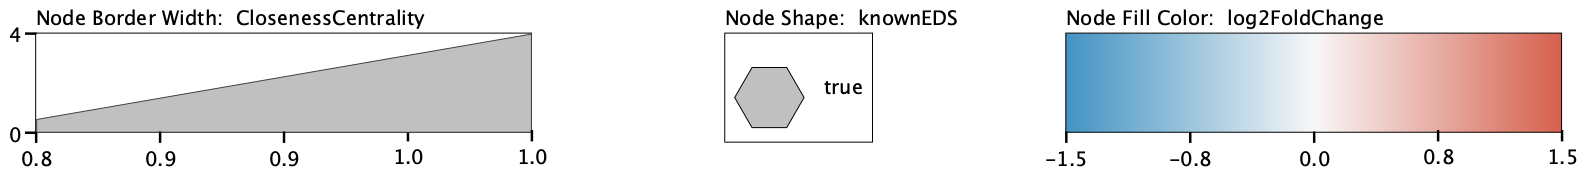
\includegraphics[width=\textwidth]{fig/mcode-legend.png}
 		\vspace{0.2cm}
 	\end{subfigure}
	\begin{subfigure}{.49\textwidth}
		\centering
 		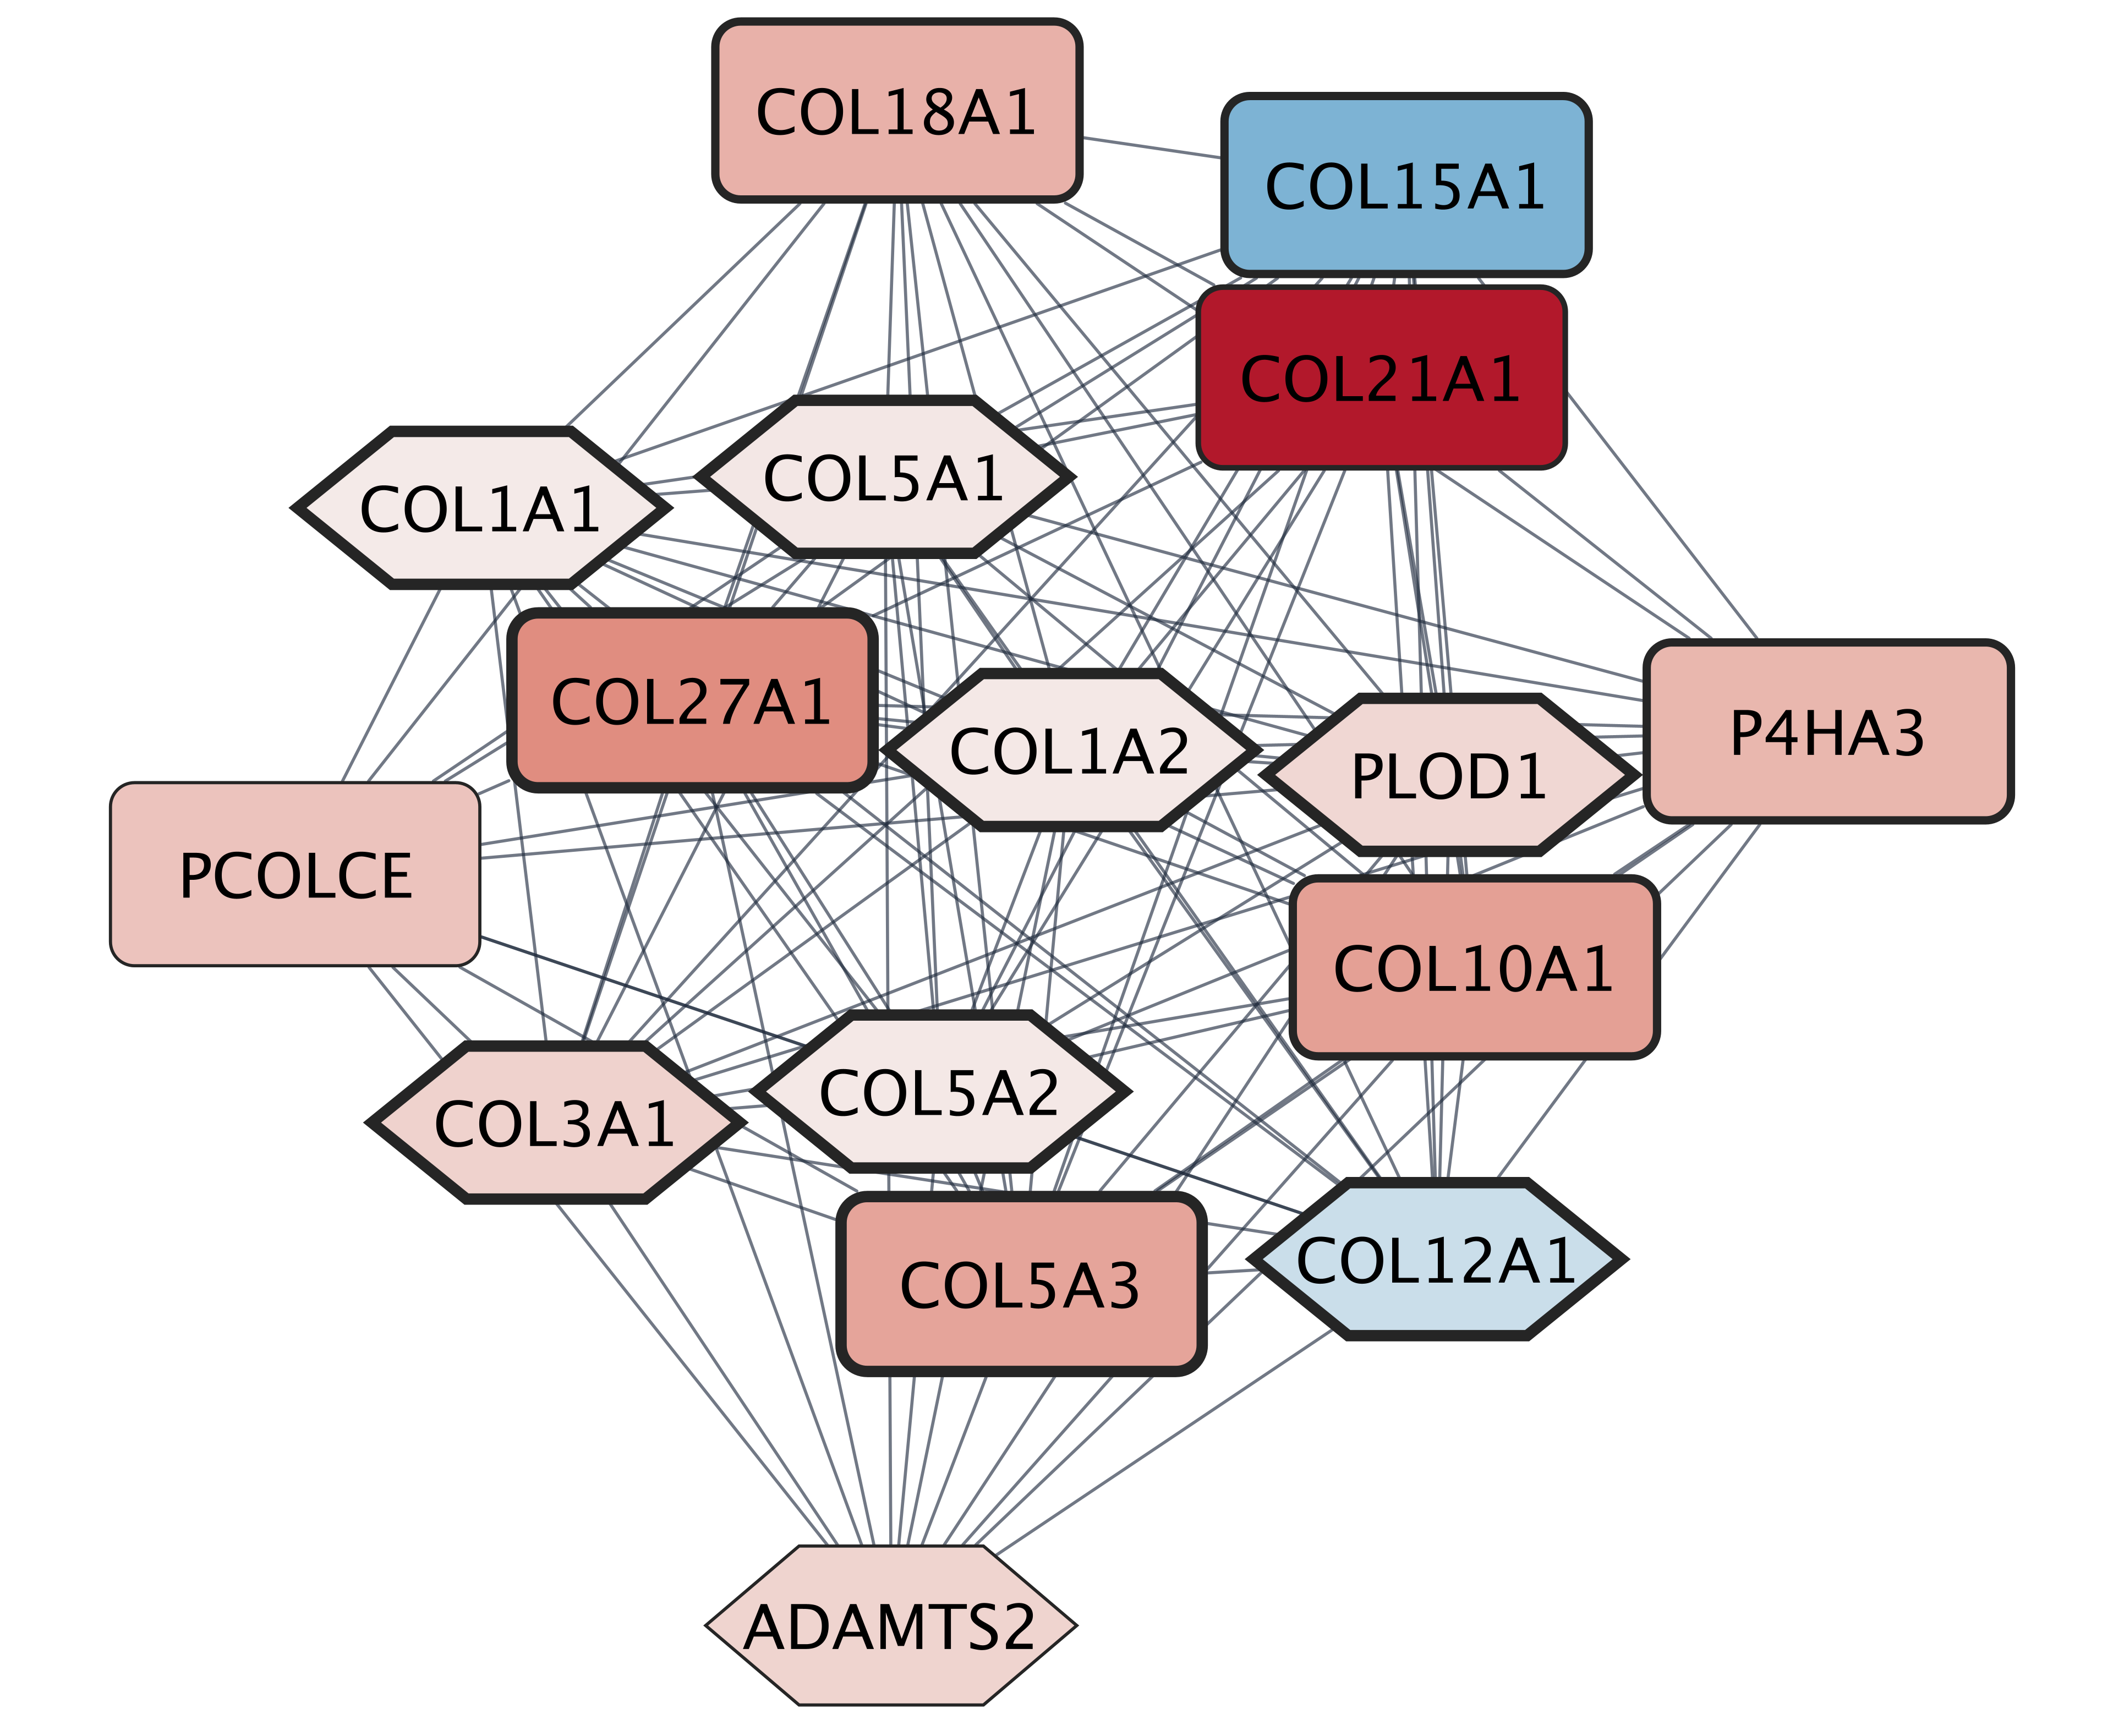
\includegraphics[width=\textwidth]{fig/mcode-cluster-without-enrichment.png}
 			\caption{Without visualisation of the ECM GO-term}
 	\end{subfigure}
 	\begin{subfigure}{.49\textwidth}
 		\centering
 		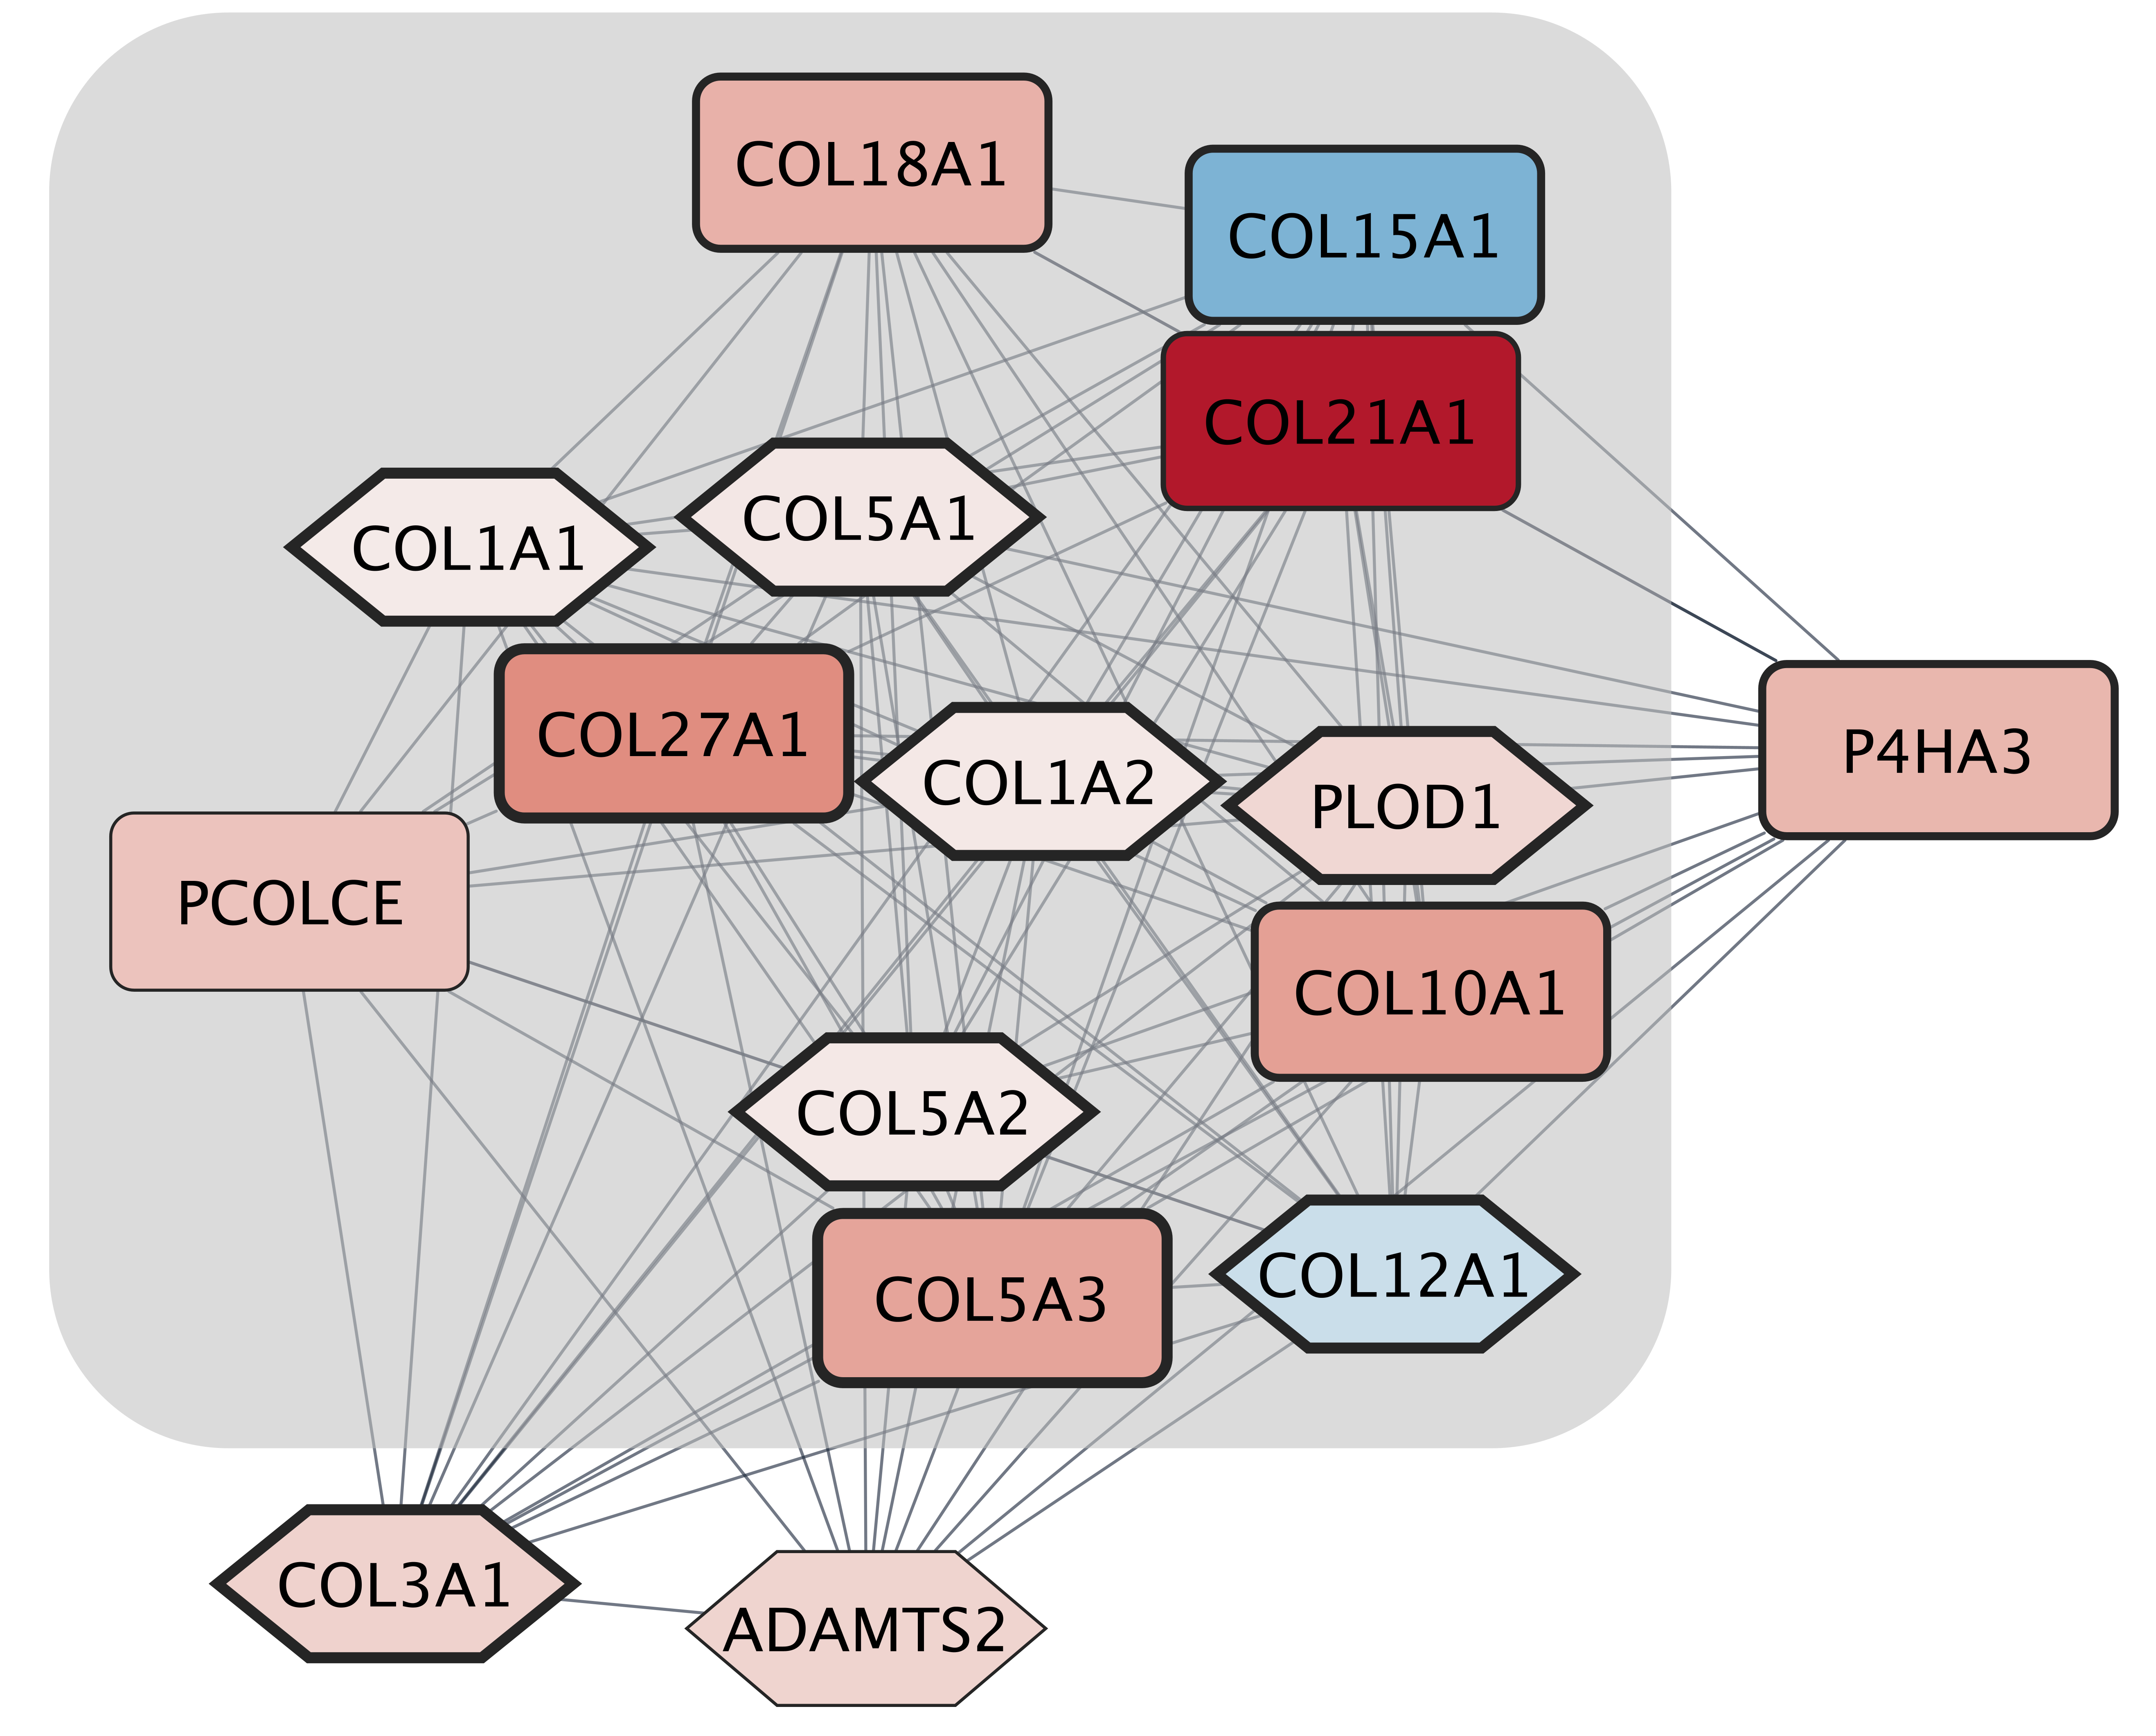
\includegraphics[width=\textwidth]{fig/mcode-cluster-eds-genes-with-ecm.png}
 		\caption{With visualisation of the ECM GO-term}
 	\end{subfigure}
	\caption[MCODE cluster with EDS genes]{\centering The MCODE cluster contains many genes known to cause other types of EDS.}
	\label{fig:mcode3}
\end{figure}

GO-Enrichment testing over-representation of molecular functions of the cluster returns two GO terms related to the extracellular matrix, GO:0005201 and GO:0030020, with the second one being a subterm of the first. Both GO terms contain the same EDS genes and seven, respectively, six other genes, with PCOLE being the only one not present in the subterm. The collagen-related genes COL27A1 and COL5A3 have a central position in the cluster and relatively strong differential expression. The gene COL21A1 is very strongly differentially expressed ($\text{log2FoldChange} > 2$), more than twice as high as the other genes, while being less central. The collagen encoded by this gene maintains the integrity of ECM and is a paralog to COL5A1, a known EDS gene \cite{COL21A1}. The deficiency of the collagen type encoded by COL15A1, the only significantly down-regulated gene, is associated with muscle and microvessel deterioration in mice. This gene is a paralog of COL5A1 as well.

Finding connections to ECM in the enrichment analysis is consistent with similar research \cite{Ritelli2022, Gensemer2021, Chiarelli2018}. Although the connection of the ECM is already known, the visualisation provided in Figure \ref{fig:mcode3} allows us to assess the centrality together with the differential expression, letting the before-mentioned genes stand out.

\paragraph{Up-regulated MCODE Clusters.} The two larger, up-regulated MCODE clusters show no relation to ECM terms, as is shown in Figure \ref{fig:mcode-cluster-mf}. It is noticeable that only a few genes of the first cluster are part of the enriched terms, while the gene ratio is much higher for the second cluster, with up to around 80\,\% of the genes being involved in the first two terms. Therefore, the enrichment of the first cluster provides little insight into molecular function in hEDS patients. On the other hand, the up-regulation seen in the second cluster for the GO-term GO:0030527, the structural constituent of chromatin, is interesting because earlier research found down-regulated genes involved in processes related to chromatin in vEDS \cite{Chiarelli2018}.

 \begin{figure}[htb!]
 	\centering
 	\caption*{\textbf{Molecular function enrichment for the two larger up-regulated clusters}}
		\begin{subfigure}{.49\textwidth}
			\centering
 			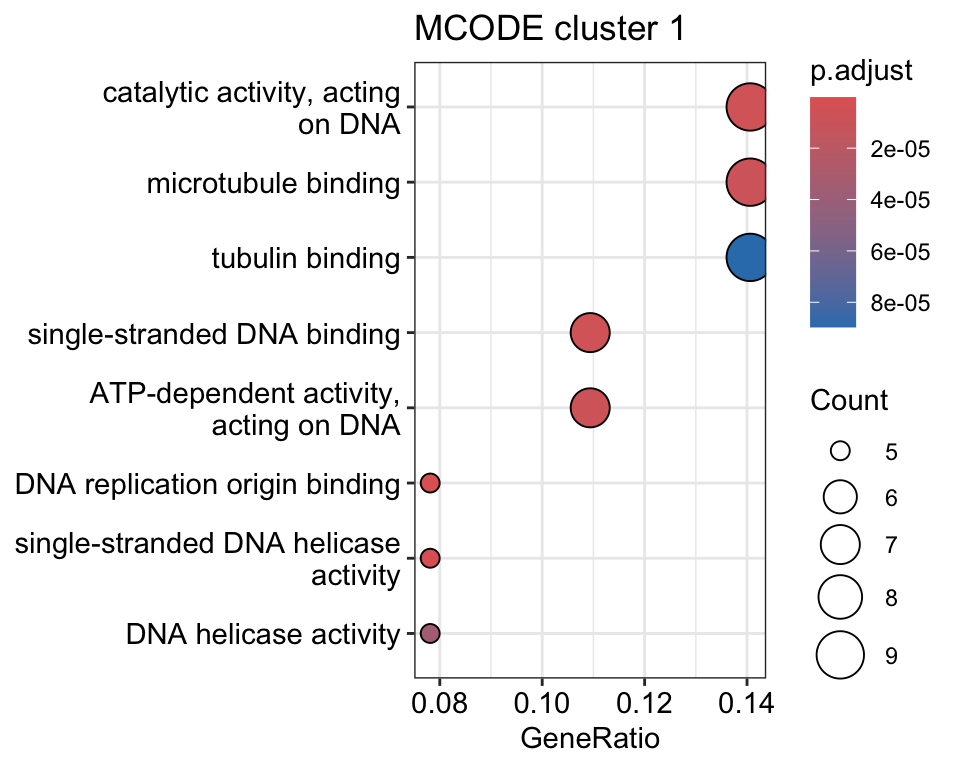
\includegraphics[width=\textwidth]{fig/mf-mcode-cluster1}
 			\caption{First MCODE cluster}
 		\end{subfigure}
    	\begin{subfigure}{.49\textwidth}
    		\centering
 			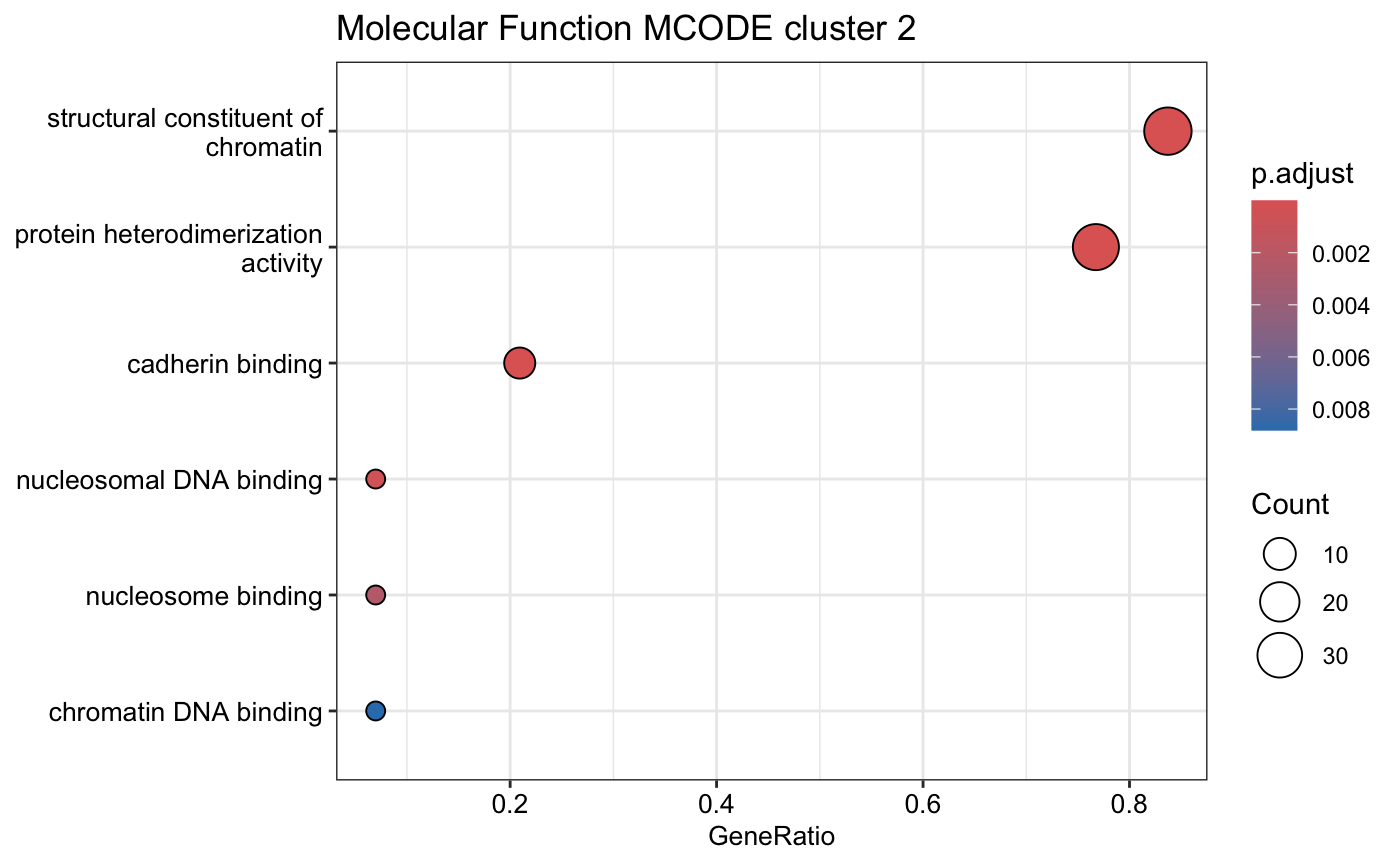
\includegraphics[width=\textwidth]{fig/mf-mcode-cluster2.png}
 			\caption{Second MCODE cluster}
 		\end{subfigure}
 	\caption{The results of the GO-enrichment for molecular function of the two up-regulated, larger MCODE clusters.}
 	\label{fig:mcode-cluster-mf}
 \end{figure}


\subsubsection{Community Clustering}

Community Clustering finds six clusters of more than 15 genes. Three are very small and loosely connected clusters containing 18 to 29 genes. These clusters are omitted from the analysis due to their small size and loose connectivity. Additionally, there are two medium-sized highly connected clusters with 76 and 105 genes and 1003 and 2330 interactions, respectively, and one huge cluster with 363 genes and 1661 interactions.

\paragraph{Medium-Sized Community Clusters.}
The medium-sized clusters are highly interconnected and contain mainly up-regulated genes. Genes related to nucleosome and protein-DNA complex are part of one of the clusters, while the genes related to the chromosomal region are clustered in the other one. This distribution is mirrored in the enriched biological processes shown in Figure \ref{fig:medium-community-bp}. In the cluster with nucleosome-related genes, five genes are notably highly up-regulated: H3C2, H3C7, H2BC10, ASF1B and WDR37. The first four are nucleosome-related, while WDR37 is related to cell cycle progression, signal transduction and gene regulation. The other cluster has no genes that are significantly more up-regulated than others.

 \begin{figure}[hbt!]
 	\centering
 	\caption*{\textbf{Biological process enrichment for the medium-sized Community Clusters}}
		\begin{subfigure}{.49\textwidth}
			\centering
 			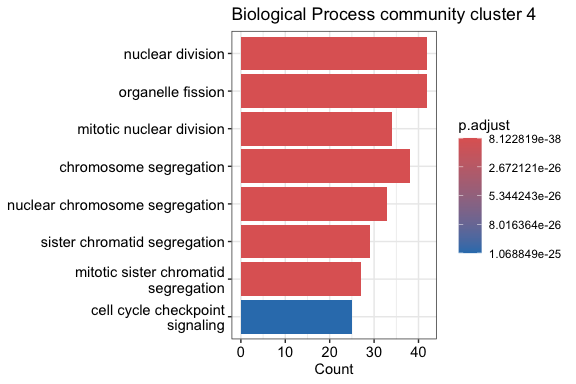
\includegraphics[width=\textwidth]{fig/Biological Process glay cluster 4.png}
 			\caption{First medium-sized Community cluster}
 		\end{subfigure}
    	\begin{subfigure}{.49\textwidth}
    		\centering
 			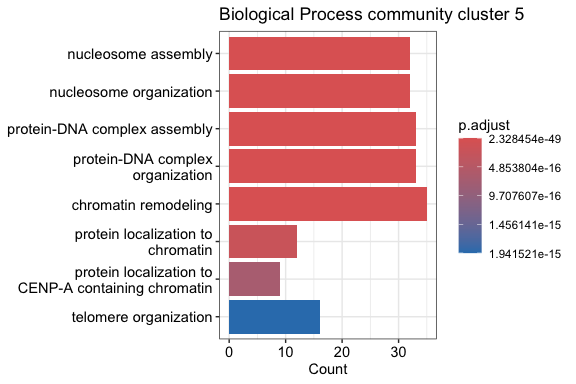
\includegraphics[width=\textwidth]{fig/Biological Process glay cluster 5.png}
 			\caption{Second medium-sized Community cluster}
 		\end{subfigure}
 	\caption{The results of the GO-enrichment for biological processes of the two medium-sized Community Clusters.}
 	\label{fig:medium-community-bp}
 \end{figure}
	%\begin{itemize}
%	\item The one with nucleosome: 5 highly differentielly expressed genes noticeable: H3C2, H3C7, H2BC10 (responsible for the nucleosome structure of the chromosomal fiber in eukaryotes), ASF1B (may play a key role in modulating the nucleosome structure of chromatin by ensuring a constant supply of histones at sites of nucleosome assembly), WDR37 (Members of this family are involved in a variety of cellular processes, including cell cycle progression, signal transduction, apoptosis, and gene regulation)
%	\item the other one more homogenous, no genes that are significantly more up-regulated than others
%\end{itemize}
\paragraph{Largest Community Cluster.} 
The largest cluster contains a mix of up-regulated and down-regulated genes and all 21 EDS-related genes. Furthermore, it contains all  genes being part of the GO-term for the ECM found in the over-representation of molecular functions of the MCODE cluster containing the EDS genes. The molecular cluster showing enrichment towards the chromatin part is not a part of this community cluster. Heat Diffusion starting at EDS genes finds 39 DEGs with a heat $> 0.1$ beside the starting nodes. These hot genes intersect with the MCODE cluster containing the EDS genes, as expected due to their close connection reflected in the clustering. Besides those, there are 31 hot genes, showing that the EDS genes have a central position close to ECM-related genes. GO enrichment of the hot genes not intersecting with the EDS-related MCODE cluster shows an ECM relation as well.
	% CLEC3B, LAMA5, MAN1B1, PLS3, TNC, ADAMTS4, LAMB3, LAMB1, SLC4A11, MYLK, MKX, OGN, LOXL4, ASPN, MYH11, OLFML2B, COMP, C4B, HS6ST1, FNDC1, INHBA, CHPF, LOXL1, GPC4, NUDCD1, ADAMTSL4, CSPG4, SULF1, NETO2, CNIH3, ITGBL1

\subsection{Conclusion}

The analysis is consistent with previous research in finding DEGs that influence the extracellular matrix, chromatin, nucleosome and the cell cycle \cite{Chiarelli2018, Ritelli2022}. Furthermore, clustering revealed which differentially expressed genes are closely related to the ones causing other EDS types. By providing a visualisation of the involvement in the extracellular matrix by simultaneously providing information about the differential expression, genes of particular interest can be identified. These results are complemented by using Heat Diffusion in the largest Community Cluster containing EDS-related genes. % It particularly shows that some gene candidates identified in earlier research are closely related to other EDS causing genes [TODO: source].

Moreover, clustering revealed that mainly up-regulated genes are closely connected; partially overlapping clusters were found by MCODE and Community Clustering. Some of the related GO terms are known to be involved in other EDS types and to involve down-regulated genes there are up-regulated in the given data. Generally, hEDS has a broad spectrum of clinical representations that might be caused by multiple components being involved as part of the molecular cause. This spectrum is reflected in the found clusters representing different processes involved.

Clear candidate genes cannot be provided although affected biological processes are identified and genes of interest described. Future work should include results from pathway analysis and analyse the created network with the found clusters in more detail.
%[TODO: list some particular interesting genes]

%\begin{itemize}
%	\item ECM/collagen in genes closely related to genes of other EDS types, seen in community cluster and MCODE cluster
%	\item TODO: link to research, meaning
%	\item chromatin related terms in a MCODE cluster and a community cluster found, in community cluster together with nucleosome
%	\item chromatin interesting because down-regulated in other EDS type
%	\item TODO: link to research, meaning
%	\item heat diffusion in largest community cluster showed other genes additionally to ECM genes that are probably interesting
%	\item project showed genes fullfilling similar roles than genes in other EDS types, candidates for causing hEDS
%	\item hEDS has wide spectrum of representations, probably multiple components represented in the found clusters
%\end{itemize}

% all chromatin genes in Community cluster 5